\documentclass[a4paper,12pt]{article}
\usepackage[utf8]{inputenc}
\usepackage{color}
\usepackage{url}
\usepackage[T2A]{fontenc}
\usepackage{graphicx}

\usepackage[english,serbian]{babel}

\begin{document}

\title{Zene u programiranju\\ \small{Seminarski rad u okviru kursa\\Tehnicko i naucno pisanje\\ Matematicki fakultet}}

\author{Jelena Velickovic\\ mi21203@alas.matf.bg.ac.rs \and\and Bojana Zagorac\\ mi22135@alas.matf.bg.ac.rs \and\and Milos Bigovic\\ \and\and\and Zorana Jevtic\\}

\date{Novembar 2022.}

\maketitle

\begin{abstract}
    U ovom tekstu je ukratko objasnjen doprinos zena u programiranju uz priloge. Takodje, bice reci o
    brojnosti zena koje se time bave, kao i o Adi Bajron, najistaknutijom zenom programerom. Sustina 
    ovog teksta je razbijanje predrasude da se programiranjem bave iskljucivo muskarci, odnosno da je 
    programiranje "muski posao". 
\end{abstract}

\flushleft\section{Sadrzaj}
\tableofcontents

\newpage
\section{Uvod}

\newpage
\section{Ada Bajron}

\begin{figure}
    \centering
    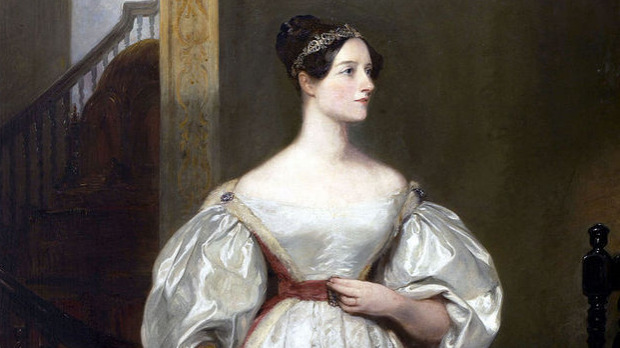
\includegraphics[width = \textwidth]{figs/adabajron.jpg}
    \caption{Ada Bajron}
    \label{fig:my_label}
\end{figure}


\end{document}
